\documentclass[tikz,border=2pt,11pt]{standalone}
\usetikzlibrary{arrows.meta}
\usetikzlibrary{positioning}
\usetikzlibrary{calc}
\usepackage{amsmath}
\usepackage{amssymb}
\usepackage{tikz}
\usepackage{xcolor}
\newcommand{\TV}{\mathrm{TV}}
\newcommand{\op}{\mathrm{op}}
\newcommand{\HS}{\mathrm{HS}}
\newcommand{\E}{\mathbb E}
\newcommand{\one}{\mathbf1}
\newcommand{\id}{\mathrm{id}}
\DeclareMathOperator{\sgn}{sgn}
\DeclareMathOperator{\tr}{tr}
\begin{document}
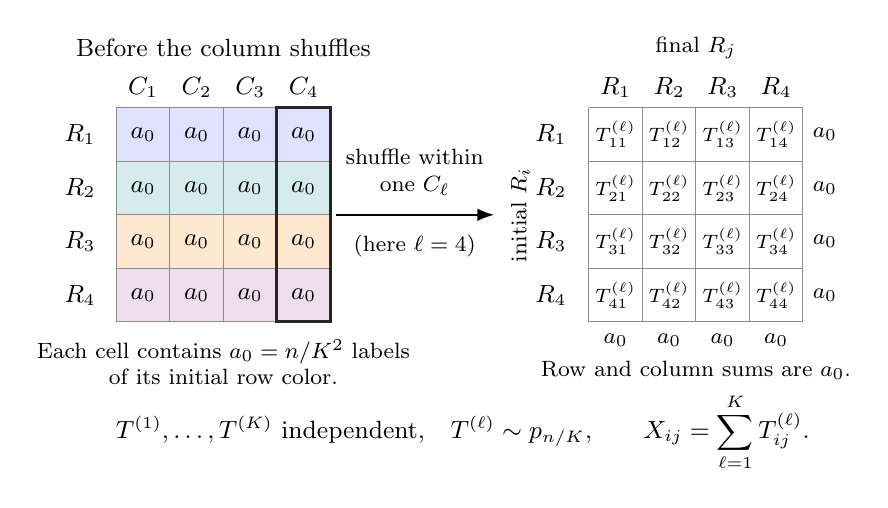
\begin{tikzpicture}[
  x=1cm,y=1cm,>=Latex,
  every node/.style={font=\small},
  gridline/.style={draw=black!45,line width=.35pt},
  tableentry/.style={font=\scriptsize},
  note/.style={font=\footnotesize}
]
  \foreach \row/\tone in {1/blue!12,2/teal!16,3/orange!18,4/violet!13} {
    \pgfmathsetmacro{\yb}{(4-\row)*.68}
    \fill[\tone] (0,\yb) rectangle (2.72,\yb+.68);
    \node[anchor=east] at (-.14,\yb+.34) {$R_{\row}$};
    \foreach \col in {1,...,4} {
      \pgfmathsetmacro{\xc}{(\col-.5)*.68}
      \node at (\xc,\yb+.34) {$a_0$};
    }
  }
  \foreach \line in {0,...,4} {
    \draw[gridline] (\line*.68,0)--(\line*.68,2.72);
    \draw[gridline] (0,\line*.68)--(2.72,\line*.68);
  }
  \foreach \col in {1,...,4} {
    \node at ({(\col-.5)*.68},2.98) {$C_{\col}$};
  }
  \draw[black!85,line width=1.1pt] (2.04,0) rectangle (2.72,2.72);
  \node at (1.36,3.48) {Before the column shuffles};
  \node[note,align=center] at (1.36,-.51)
    {Each cell contains $a_0=n/K^2$ labels\\of its initial row color.};

  \draw[->,line width=.7pt] (2.79,1.36)--(4.80,1.36);
  \node[note,align=center] at (3.79,1.90) {shuffle within\\one $C_\ell$};
  \node[note] at (3.79,.97) {(here $\ell=4$)};

  \foreach \row in {1,...,4} {
    \pgfmathsetmacro{\yb}{(4-\row)*.68}
    \node[anchor=east] at (5.84,\yb+.34) {$R_{\row}$};
    \foreach \col in {1,...,4} {
      \pgfmathsetmacro{\xc}{6.00+(\col-.5)*.68}
      \node[tableentry] at (\xc,\yb+.34) {$T^{(\ell)}_{\row\col}$};
    }
    \node[note] at (9.00,\yb+.34) {$a_0$};
  }
  \foreach \line in {0,...,4} {
    \draw[gridline] (6.00+\line*.68,0)--(6.00+\line*.68,2.72);
    \draw[gridline] (6.00,\line*.68)--(8.72,\line*.68);
  }
  \foreach \col in {1,...,4} {
    \node at ({6.00+(\col-.5)*.68},2.98) {$R_{\col}$};
    \node[note] at ({6.00+(\col-.5)*.68},-.23) {$a_0$};
  }
  \node[rotate=90,note] at (5.13,1.36) {initial $R_i$};
  \node[note] at (7.36,3.48) {final $R_j$};
  \node[note] at (7.36,-.62) {Row and column sums are $a_0$.};

  \node[align=center] at (4.40,-1.40)
    {$T^{(1)},\ldots,T^{(K)}$ independent,\quad
      $T^{(\ell)}\sim p_{n/K}$,\qquad
      $X_{ij}=\displaystyle\sum_{\ell=1}^{K}T^{(\ell)}_{ij}$.};
\end{tikzpicture}
\end{document}
